% sudo apt install texlive-latex-base texlive-lang-cyrillic texlive-latex-recommended texlive-latex-extra
% pdflatex Polyarniy_CV.pdf

\documentclass[11pt,oneside]{article}
\usepackage[utf8]{inputenc}
\usepackage[english,russian]{babel}
\usepackage{xcolor}
\usepackage{hyperref}
\usepackage[left=2.5cm,right=2.5cm,top=2.5cm,bottom=2.5cm]{geometry}

% to fix last word in the line (so that it will not be out of the right border)
\usepackage{microtype}
\sloppy

\usepackage{graphicx}
\usepackage{wrapfig}
\usepackage[absolute,overlay]{textpos}
\graphicspath{ {imgs/} }

\newcommand{\hhref}[2]{\href{#1}{\color{blue}#2}}

\begin{document}

% \begin{textblock}{7}(9.0,0.3)
%     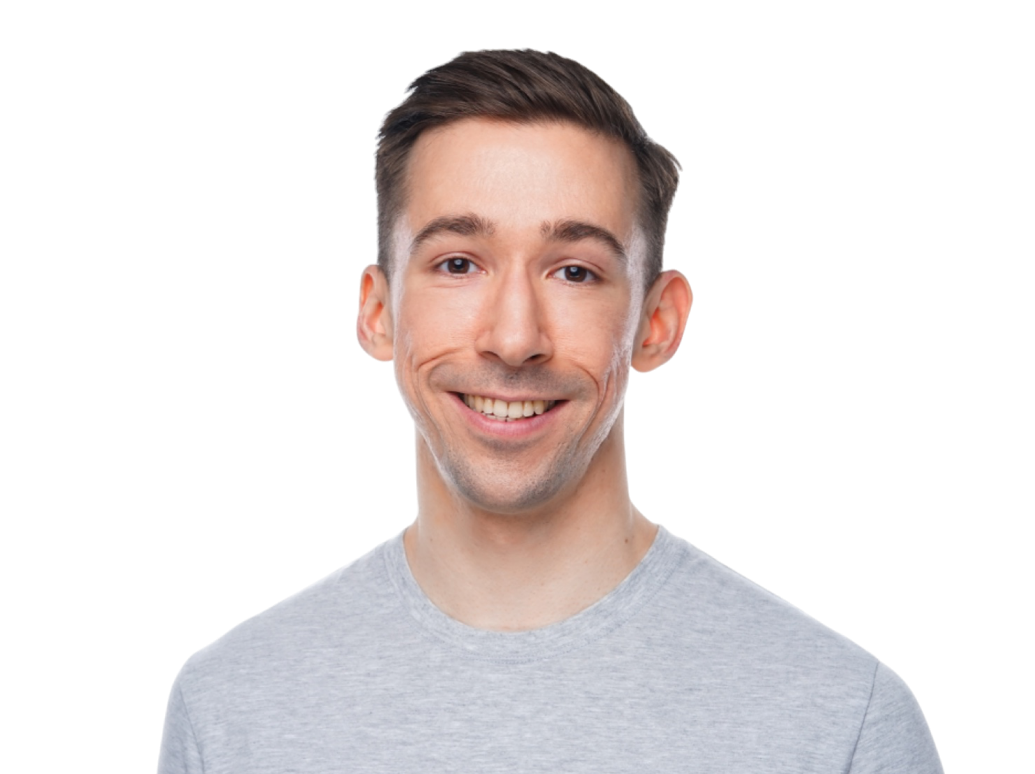
\includegraphics[scale=0.45]{photo2025.png}
% \end{textblock}
\begin{wrapfigure}{r}{0.35\textwidth}
  \vspace{-80pt}
  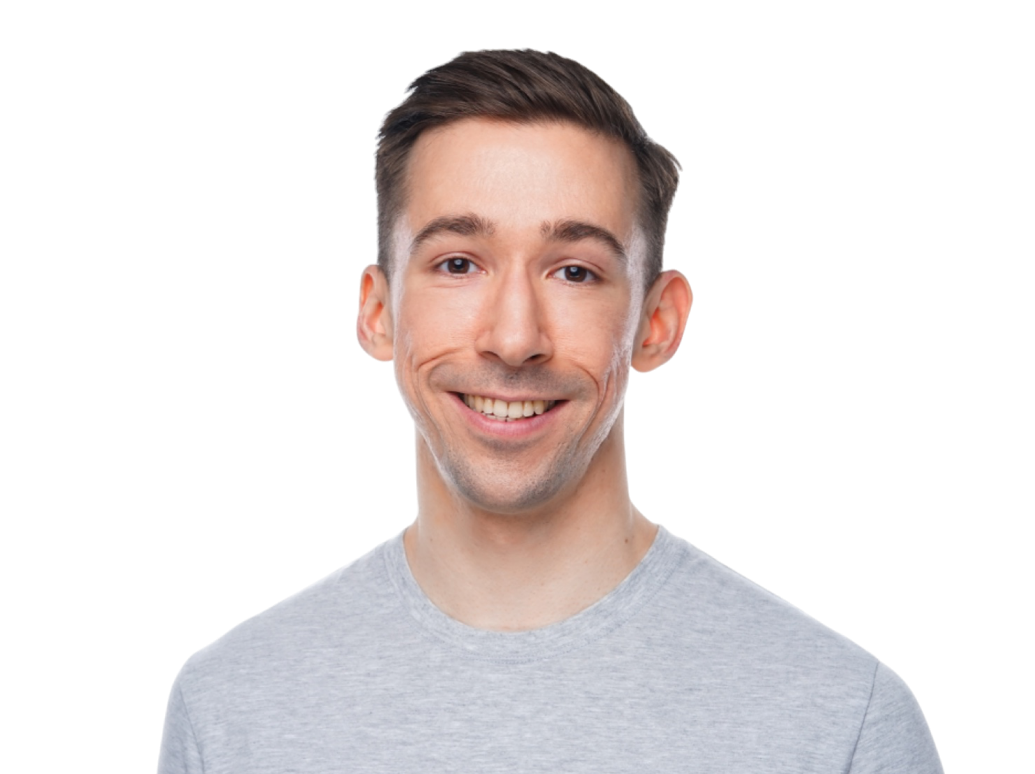
\includegraphics[width=0.35\textwidth]{photo2025.png}
  \vspace{-10pt}
\end{wrapfigure}

\begin{center}
        {\huge Nikolai Poliarnyi}
	%{\huge Poliarnyi Nikolai \\ Полярный Николай}
\end{center}

Expert in photogrammetry, 3D computer vision, computational geometry, GPU programming (Vulkan, CUDA, OpenCL), teaching and 'fixing things'. Inventor of breakthrough algorithms published at top-tier venues (ICCV) and presented at international conferences (ISPRS). Passionate about pushing the boundaries of what's possible in computer vision and GPGPU.
%A strong technical leader with deep empathy and a talent for making complex topics accessible — both in mentoring teams and teaching at top universities and schools.

\vspace{-9pt}
\section*{\textbf{Work Experience}}
\vspace{-9pt}


\begin{description}

  \item[ - \hhref{https://en.wikipedia.org/wiki/PhotoScan}{Agisoft Metashape}] - \textbf{Since April 2016}

    \textbf{Principal Research Engineer (Team Lead)}

    Computer Vision, Computational Geometry, OpenCL/CUDA/Vulkan, LiDAR, AI/ML

    One of the world's leading photogrammetry solutions. Supports Windows, Linux, and macOS, with GPU accelerated computations on NVIDIA, AMD, Intel, and Apple Silicon.\\
    Leading high-impact innovation and performance tuning, mentoring algorithm development at scale, and resolving critical user pain points through deep technical expertise.

    \begin{itemize}

      \item Invented a new GPU-accelerated algorithm for surface reconstruction from depth maps (instead of point cloud), bridging a long-standing gap in quality and performance with industry-leading competitor Reality Capture (Epic) in a critical workflow. The method also enabled processing of city-scale scans on workstations through out-of-core data management. \hhref{https://www.polarnick.com/static/papers/poliarnyi2021.pdf}{Published a paper} at top-tier A* conference \hhref{https://openaccess.thecvf.com/content/ICCV2021/html/Poliarnyi_Out-of-Core_Surface_Reconstruction_via_Global_TGV_Minimization_ICCV_2021_paper.html}{ICCV 2021}.
      \item Invented a UAV trajectory-aware \hhref{https://www.youtube.com/watch?v=tiOeMgLHSrA}{reconstruction algorithm} that enhances the detail of Digital City Twin models reconstruction from aerial LiDAR scans and makes combined processing from images, aerial LiDAR, and terrestrial LiDAR possible. Presented the report \hhref{https://polarnick.com/static/presentations/AgisoftMetashapeGSW2023.pdf}{‘LiDAR and Photogrammetry Compared and Combined‘} at the ISPRS GSW 2023 Conference.
      \item Invented an OpenCL/CUDA-accelerated depth reconstruction algorithm that solves critical challenges in 3D scanning — such as the reconstruction of thin railings and specular or reflective surfaces. The method also supports Multi-GPU acceleration and builds faster and cleaner results compared to previous methods.
      \item Invented a novel Vulkan-accelerated texturing algorithm that solves critical challenges: optimizing texture atlas fill ratio, automatically ignoring out-of-focus image regions, and filtering transient objects (e.g., passing cars, pedestrians). The method is out-of-core, making it suitable for consumer-grade PCs.
      \item Designed and delivered a comprehensive \hhref{https://www.youtube.com/playlist?list=PL5p-5hHpsHBp4yTpeZJ_QMSmJPAuov-VF}{photogrammetry training program} to develop and recruit top-tier talents among students (CS Club, CS Center, SPbU, ITMO).
      \item User-centered roadmap planning via direct community feedback from niche platforms (industry forums, Reddit, \hhref{https://github.com/agisoft-llc/metashape-scripts}{GitHub}). Monitoring competitor product updates and conducting regular performance benchmarking.
      \item Developed innovative engineering methodologies to accelerate algorithm development, improve interpretability and maintainability, and simplify debugging. This includes techniques to quickly identify when user-side issues stem from hardware instability rather than software bugs.
      \item Developed wrappers for OpenCL/CUDA/Vulkan APIs.
      \item Enhanced cloud performance, achieving 2x faster processing.
      % \item Photographed (15K images) and digitized the UNESCO site \hhref{https://heritage3d.ru/models/kizhskiy-pogost}{Kizhi Pogost}.
      % \item Deployed an on-premises LLM server to enable secure AI-assisted development.
    \end{itemize}
  \item[ - Transas] - 2014 - 2016 - Mathematician-Programmer %% \textbf{October 2014 - March 2016}

    OpenCV, OpenCL, Python, Cython, Ceres-solver

    Developed a server that produces 3D landscape reconstruction and true orthophoto stitching from UAVs' data.
    % (\hhref{http://polarnick239.github.io/old/cv/Monoceros1.pdf}{presentation}, \hhref{http://polarnick239.github.io/old/cv/Monoceros2.pdf}{second presentation}).

  \item[ - Yandex.Money] - 2014 - Software Developer (Java backend) %% \textbf{February 2014 – October 2014:}
  \item[ - DevExperts] - 2013 - Software Developer (Java backend) %% \textbf{April 2013 – September 2013:}

\end{description}


\vspace{-9pt}
\section*{\textbf{Skills}}
\vspace{-9pt}

\begin{itemize}
    \item{\textbf{Computer Vision}}: Structure from Motion, Multiple View Geometry, AI/ML, object detection, classification, and segmentation. Developed state-of-the-art algorithms for depth map estimation, surface reconstruction, and texturing, outperforming existing solutions.

    \item{\textbf{\hhref{https://github.com/GPGPUCourse/GPGPUVulkan}{Vulkan}, OpenCL, CUDA, OpenGL, WebGL}}: State-of-the-art algorithms of arbitrary complexity. Profiling, accelerating, and adapting algorithms for the GPU. Experienced in working around GPU driver bugs. \hhref{https://youtu.be/zJ6ru8dNAcs?t=5698}{Explored} DeepSeek’s fine-grained quantization method, which demonstrated a 2x reduction in training costs in their implementation. \hhref{https://www.youtube.com/watch?v=ltUzX1IR9JI&list=PL5p-5hHpsHBolSeDn7__1c9hgPprYTjnn&index=3}{Explored} algorithms behind Unreal Engine 5 Nanite tech.

    \item{\textbf{Computational geometry, CGAL}}: computations with absolute accuracy, algorithms and structures like Delaunay triangulation.

    \item{\textbf{Teaching}}: deep empathy and a talent for making complex topics accessible — both in mentoring teams and teaching at top universities and schools.

    \item{\textbf{C++, Python, Java}}
\end{itemize}

\vspace{-9pt}
\section*{\textbf{Education}}
\vspace{-9pt}

\begin{itemize}
    \item{Computer Science Center}
    \item{ITMO University, Computer Technologies}
    \item{PML №239, mathematical circle, programming contests}
\end{itemize}


\vspace{-9pt}
\section*{\textbf{Other Activities}}
\vspace{-9pt}

\begin{itemize}
    \item{\textbf{Photogrammetry course}}: developed Photogrammetry  \hhref{https://compsciclub.ru/courses/photogrammetry/2021-spring/}{course} for the Computer Science Club. Teaching it in \hhref{https://math-cs.spbu.ru/}{SPbU} and \hhref{https://ct.itmo.ru/}{ITMO}.  \hhref{https://www.youtube.com/watch?v=rEF0zkv2cn8&list=PL5p-5hHpsHBp4yTpeZJ_QMSmJPAuov-VF&index=1}{Video recordings}. Tasks on \hhref{https://github.com/PhotogrammetryCourse/}{github}.

    \item{\textbf{GPGPU course}}: developed GPGPU OpenCL \hhref{https://compscicenter.ru/courses/video_cards_computation/}{course} in Computer Science Center. \hhref{https://www.youtube.com/watch?v=LDt4KQEdImY&list=PLlb7e2G7aSpSkDWlyJQzT9Qx9rrgKSgAp&index=1}{Video recordings}. Tasks on \hhref{https://github.com/GPGPUCourse/}{github}.

    \item{\textbf{Conferences}}: published \hhref{https://www.polarnick.com/static/papers/poliarnyi2021.pdf}{a paper} on \hhref{http://iccv2021.thecvf.com/}{ICCV 2021}. Presented the report \hhref{https://polarnick.com/static/presentations/AgisoftMetashapeGSW2023.pdf}{‘LiDAR and Photogrammetry Compared and Combined‘} at the ISPRS GSW 2023 Conference. Participated in \hhref{http://3dv18.uniud.it/}{3DV 2018} and \hhref{http://www.3d-arch.org/}{3D-ARCH 2019}.

    \item{\textbf{Public lectures}}: \hhref{https://csspace.io/open-lecture/2025-gpu}{GPGPU in CS Space}, \hhref{https://www.youtube.com/watch?v=adQQoH3iXPQ}{Science Day in school}, \hhref{https://www.youtube.com/watch?v=ltUzX1IR9JI&list=PL5p-5hHpsHBolSeDn7__1c9hgPprYTjnn&index=3}{Algorithms behind Unreal Engine 5 Nanite tech}.

    \item{\textbf{Consultant}}: provide consulting and project development services to companies and startups on topics related to Computer Vision and GPU acceleration.

    \item{\textbf{Open-source}: \hhref{https://github.com/GPGPUCourse/GPGPUVulkan}{Vulkan API library}. \hhref{https://github.com/PolarNick239/ExternalSortingOnGPU}{Out-of-core merge sort} with GPU acceleration. \hhref{https://gist.github.com/PolarNick239/7819fb7722fab09b37ecaee77c82cf58}{96-bit 3D Morton code}. OpenCL \hhref{https://github.com/PolarNick239/OpenMeanShift}{implementation} of EDISON mean shift. \hhref{https://github.com/opencv/opencv/pull/6078}{Implemented} Python bindings for OpenCL algorithms in OpenCV. Contributions to OpenCV, PyOpenCL, jupyter qtconsole and others. GPU monitoring in i3pystatus.}

    \item{\textbf{Hackathons}}: 6 awards at hackathons. Two first places on \hhref{https://github.com/PolarNick239/HackathonDroneSwarm}{X-Mas Hack} (mission planner for drone swarm). Third place at \hhref{https://career.luxoft.com/lp/hack-cv/}{HackCV} (traffic sign recognition), \hhref{http://hackday.ru/sciencehackday-2/projects\#project-1400}{Science Hackday \#2} (Startup nomination), \hhref{http://hackday.ru/hackday-36/projects\#project-1121}{Hackday\#36} (Autodesk 3D-web nomination), \hhref{https://www.hackerleague.org/hackathons/jetbrains-edtech-hackathon/blogposts/53655896e24d32cfbd000006}{HackEdu} by JetBrains (third place). Participation in \hhref{http://www.hackjunction.com/}{Junction 2016, 2017}.

    \item{\textbf{Magister Ludi}}: \hhref{http://239.ru}{PML №239} programming teacher. Supervise over 20 student game development \hhref{https://www.youtube.com/watch?v=bbKXnsysUXw}{projects} annually.
\end{itemize}

\begin{wrapfigure}{r}{0.22\textwidth}
    \centering
    \includegraphics[width=0.22\textwidth]{unicorn.png}
\end{wrapfigure}

\vspace{-9pt}
\section*{\textbf{Contacts}}
\vspace{-9pt}

\begin{itemize}

    \item{\textbf{\hhref{mailto:PolarNick239@gmail.com}{PolarNick239@gmail.com}}}

    \item{\textbf{\hhref{https://t.me/polarnick239}{Telegram}}}

    \item{\textbf{\hhref{https://www.linkedin.com/in/nikolai-poliarnyi-61393b7b}{LinkedIn}}}

    \item{\textbf{\hhref{https://github.com/PolarNick239}{GitHub}}}

    \item{\textbf{\hhref{http://polarnick239.github.io/index_ru.html}{PolarNick.ru}}}

\end{itemize}

Updated: June 07, 2025

\end{document}
